%\RequirePackage{luatex85}
\documentclass[11pt]{scrreprt}

%\usepackage{fontspec}
\usepackage{amsmath,amssymb}
\usepackage{mathpazo}
\usepackage{XCharter}
\usepackage{cabin}
\usepackage[utf8]{inputenc}
\usepackage[T1]{fontenc}
\usepackage[dvipsnames]{xcolor}
\usepackage{csquotes}
\usepackage{marginnote}
\usepackage{tikz}
\usepackage{pgfplots}
\usepackage{pgfplotstable}
\pgfplotsset{compat=newest}
\usepackage{graphicx}

\usepackage{geometry}
\usepackage[ngerman]{babel}
%\defaultfontfeatures{Ligatures=TeX}
% Set sans serif font to Calibri
%\setsansfont{Calibri}
% Set serifed font to Cambria
%\setmainfont{Cambria}
% Define light and dark Microsoft blue colours
\definecolor{MSBlue}{rgb}{.204,.353,.541}
\definecolor{MSLightBlue}{rgb}{.31,.506,.741}
\addtokomafont{chapter}{\color{MSBlue}}
\addtokomafont{section}{\color{MSBlue}}
\addtokomafont{subsection}{\color{MSLightBlue}}

\addtokomafont{caption}{\sffamily}
\addtokomafont{captionlabel}{\usekomafont{caption}\bfseries\color{MSBlue}}

\usepackage[backend=biber,style=authortitle,hyperref=true,backref=true,block=none,url=false,isbn=false,doi=false,maxcitenames=3,maxbibnames=100]{biblatex}
\addbibresource{references.bib}

\title{Ganz bunt-Die Verwendung von Farbstoffen in Lebensmitteln}
\author{Lukas Braun}
\publishers{\includegraphics[width=5cm]{logo.jpg} \\ Descartes Gymnasium Neuburg a. d. Donau}
\subject{Biologie}
\subtitle{W-Seminar -- Kochen genießen verstehen-Biochemie und Herstellung von Lebensmitteln}
\date{07. Oktober 2016}

\usepackage[automark]{scrlayer-scrpage}
\usepackage[onehalfspacing]{setspace}
\emergencystretch=.5em
\renewcommand*{\dictumauthorformat}[1]{(#1)\vspace*{1em}}



\makeatletter

\newrobustcmd*{\parentexttrack}[1]{%
	\begingroup
	\blx@blxinit
	\blx@setsfcodes
	\blx@bibopenparen#1\blx@bibcloseparen
	\endgroup}

\AtEveryCite{%
	\let\parentext=\parentexttrack%
	\let\bibopenparen=\bibopenbracket%
	\let\bibcloseparen=\bibclosebracket}

\makeatother



\usepackage{siunitx}

\usepackage{abstract}
\setlength{\absleftindent}{3cm}
\setlength{\absrightindent}{3cm}
\setlength{\absparindent}{0cm}

\usepackage[hidelinks]{hyperref}

\AtBeginDocument{\addtocontents{toc}{\protect\thispagestyle{empty}}}

 
\begin{document}
\pagestyle{empty}
\renewcommand{\abstractname}{Abstract}
\maketitle
\pagestyle{empty}
\clearpage
\newgeometry{
	a4paper,
	left=30mm,
	right=20mm,
	top=25mm,
	bottom=25mm
}

\begin{abstract}
	\noindent

\end{abstract}
\pagestyle{empty}
\clearpage
\pagestyle{empty}
\tableofcontents
\clearpage
\pagestyle{empty}
\begingroup
\makeatletter
\let\ps@plain\ps@empty
\makeatother

\pagestyle{empty}
\listoffigures
\cleardoublepage
\endgroup
\clearpage
\pagestyle{headings}


\chapter{Geschichte der Lebensmittelfarben}
Auch Menschen reagieren sehr stark auf die Farben der Umwelt, so verbinden wir ein bestimmtes Lebensmittel meist mit genau einer Farbe. Denn wer assoziiert Himbeeren mit einer anderen Farbe als einem leuchtenden Rot? Dieses Verhalten hat sich im Menschen über Jahrtausende durch Traditionen und der Umwelt eingeprägt. Auch heute noch wird bei einem Einkauf zunächst die Farbe der Lebensmittel überprüft. Sie gibt die Reife und somit eine Erwartung an Geschmack, Geruch und Inhaltsstoffe an. Deshalb werden zur Entwicklung von modernen Lebensmitteln bereits Farbpsychologen benötigt und in einem Supermarkt die Früchte mit speziellem Licht bestrahlt, um sie für den Kunden ansprechender wirken zu lassen\parencite{Hamatschek.2016}.
Wie die Farbe der Lebensmittel uns Menschen beeinflusst zeigt sich am folgenden Beispiel: So werden rot gefärbte Süßigkeiten laut einer Studie für den Menschen süßer wahrgenommen als andersfarbige Süßigkeiten. Die Farben Grün und Gelb wiederum werden mit einem saurem Geschmack assoziiert. Eine weitere relativ bekannte Studie nutzte diese Erwartungshaltung des Menschen aus, indem ein rot gefärbter Naturjoghurt von den Testpersonen mit unterschiedlichen Geschmacksrichtungen, wie Erdbeere oder Kirsche, verbunden worden ist.
%http://www.bbc.com/future/story/20160226-why-bowl-food-might-be-tricking-your-brain
%aufgerufen am 02.11.2016
%http://www.berliner-zeitung.de/wissen/essen-wie-farbe-den-geschmack-manipuliert-22524546

Diese Phänomene werden seit einer langen Zeit von Menschen benutzt.Bereits um 1500 vor Christus färbten ägyptische Händler ihre Süßigkeiten, indem sie natürliche Pflanzenextrakte und Wein hinzufügten Von dort aus verbreitete sich diese Methode über das römische Reich. Diese Vorgehensweise ging im Mittelalter jedoch größtenteils verloren, da das Aussehen der Lebensmittel für die verarmte Bevölkerung vergleichsweise unbedeutend gewesen ist\parencite{HarryMeggos.1995}. Dies änderte sich erst bei Bildung von größeren Städten in der frühen Moderne. Der internationale Handel nahm zu, und es werden vermehrt exotische Gewürze und Färbemittel nach Europa importiert. So wurde bereits 1531 ein Gesetz in Augsburg erlassen, dass Fälscher von Safran mit dem Tode bestraft und allgemeine Regeln für Gewürze und Farbstoffe bestimmt.

Durch die industrielle Revolution im 19. Jahrhundert stieg die Nachfrage nach günstigen Lebensmitteln stark an. Zu dieser Zeit war die Analytische Chemie noch in ihren Kinderschuhen, sodass noch keine Lebensmittelkontrollen existierten, die den heutigen Standards ansatzweise entsprechen.  Demzufolge kann es heutzutage keinen mehr wundern, dass die Streckung von Lebensmitteln florierte. Schwermetalle und andere anorganische Stoffe stellten einen kostengünstigen Ersatz dar, um die ursprüngliche Farbe von verdünnter Milch und anderen Lebensmitteln wiederherzustellen. Mit Bleioxid können beispielsweise Käse und Süßwaren gefärbt werden\parencite{Natcol.2016,Downham.2000}.Erst im Jahre 1959 wurde in Deutschland die Farbstoff-Verordnung erlassen. Seitdem gelten in Deutschland strengere Maßstäbe bezüglich der Unbedenklichkeit von Lebensmittelzusatzstoffen. Nur noch einige Chemikalien, die auf einer Positivliste enthalten sind, dürfen noch verwendet werden. Eine weitere Verschärfung dieser Regelung erfolgte 1977 mit der Zusatzstoff-Zulassungsverordnung. Ab diesem Zeitpunkt müssen alle enthaltenen Zusatzstoffe klar deklariert sein\parencite[S.48-49]{Heinze.1986}.
Doch wie streng sind die Auflagen jetzt in Deutschland? Noch weitaus bedeutsamer ist die Frage, ob sich die Unternehmen an die auferlegten Richtlinien halten, also die richtigen Zusatzstoffe verwenden. Diese Fragen werden unter anderem in dieser Arbeit behandelt.


%Lebensmitteltechnologie Jochen Hamatschek 2016 S.88 ff
%Food colours: an international perspective von Meggos h 59 ff
%http://natcol.org/library/introduction-food-colours-legislation/ aufgerufen am 03.10.2016
%http://www.blacksci.co.uk/products/journals/freepdf/tmp1.pdf aufgerufen am 08.09.2016
%(doi:doi:10.1046/j.1365-2621.2000.00373.x. )
%http://jama.jamanetwork.com/article.aspx?articleid=465550 Artikel: Human food laws aus "The Journal of the American Medical Association. Chicago: American Medical Association." ausgabe 1898 Nr 8 von Robert W. Hastings
%http://www.fda.gov/AboutFDA/WhatWeDo/History/FOrgsHistory/CFSAN/ucm083863.htm   von U.S. Food and Drug Administration Titel: "A Century of Ensuring Safe Foods and Cosmetics"
%
\chapter{Definition von Farben}
\section{Eigenschaften }
\dictum[Sprichwort]{%
	Nachts sind alle Katzen grau.
}
 Zunächst jedoch muss erklärt werden, was es mit Farbigkeit auf sich hat. Um Farben sehen zu können, wird Licht benötigt, denn wie das Sprichwort sagt, sind nachts alle Katzen grau.  Doch was ist Licht? Um diese Frage genauer zu erklären, ist zunächst ein kleiner Exkurs in die Physik notwendig. Das \enquote{weiße} Licht der Sonne ist im Grunde eine Überlagerung von elektromagnetischer Schwingungen mit unterschiedlichen Wellenlängen $\lambda$. Hierzu betrachten wir zunächst ein Prisma aus Glas, in welchem weißes Licht aufgebrochen wird und ein Farbspektrum, vergleichbar mit einem Regenbogen, entsteht. Abhängig von der Wellenlänge wird das Licht im Prisma unterschiedlich stark gebrochen und somit das typische Farbspektrum sichtbar.  Das für den Menschen sichtbare Licht hat eine Wellenlänge zwischen \SI{400}{\nano\meter}  bei violetten Licht und \SI{800}{\nano\meter} bei rotem Licht. Die Wellenlänge des Lichtes bestimmt die Farbe und den Energiegehalt.

\begin{equation}
	E = h \frac{c}{\lambda}
\end{equation}

 So liegt die Energie des sichtbaren Lichts zwischen  \SI{1,6}{\electronvolt} bei rotem und  \SI{2,4}{\electronvolt} bei blauem Licht. Dieser Teilbereich der Physik wurde bereits in der Antike unter anderem von Ptolemäus und Archimedes erforscht.

Licht entsteht, indem zunächst Elektronen innerhalb der Atome durch die Zufuhr von Energie angeregt werden und dadurch auf eine bestimmte, höhere Energiestufe\footnote{ Entspricht einer höheren Geschwindigkeit und einer größeren Entfernung zum Atomkern} angehoben werden. Da dieser Zustand relativ energiereich und  instabil ist, fällt das Elektron auf sein ursprüngliches Energieniveau zurück. Die daraus resultierende Energiedifferenz kann, abhängig vom Molekülbau, als Wärmestrahlung oder als Lichtstrahlung abgegeben werden. Die Größe der Energiedifferenz entscheidet zudem über die Farbe des ausgesandten Lichts: Bei einer größeren Energie, wird eine kurzwelligere Strahlung emittiert.

Tritt nun Licht auf einen Körper, so können verschiedene, stoffspezifische Ereignisse auftreten: Durch diese elektromagnetische Strahlung werden Elektronen auf ihr nächsthöheres Energieniveau gehoben und beim Zurückfallen Licht ausgesandt. Dieses Phänomen wird Remission genannt. 

Eine andere Möglichkeit ist, dass nicht die genau benötigte Energiemenge an den Körper geraten und die Elektronen kein höheres Energieniveau erreichen. Die Energie wird nun nur in Form von Wärme emittiert. Jeder Stoff kann jedoch nur Licht bestimmter Wellenlängen absorbieren. Die restlichen Wellenlängen werden reflektiert, und durch additive Mischung dieser Wellenlängen resultiert die für den Menschen erscheinende Eigenfarbe des Stoffes\parencite[S.9-15]{Jenette.1983}.

\section{Färbung organischer Stoffe}

Zunächst muss der Begriff organische Stoffe definiert werden. Dies sind nahezu alle auf Kohlenstoff basierende Verbindungen. Ein einfacher Vertreter dieser Gruppe ist das farblose Methan Ch4[Strukturformel machen	].
Für die Farbigkeit sind unterschiedliche Effekte verantwortlich. Der bereits unter den Anorganischen Farbstoffen genannte Charge Transfer kann auftreten, wenn auch seltener. [fh münster]
Eine weitere Möglichkeit ist mit der Struktur eines Farbstoffes begründbar. 
So kann man hier zunächst die Strukturformeln von farblosen Benzol, schwach gelben Nitrobenzol und gelben Nitrophenol vergleichen. Trotz der relativ ähnlichen Struktur ist ein großer Farbunterschied vorhanden. 
Dies wird im Folgenden schrittweise erklärt. Das Benzol besitzt einen Sechsring mit 3 delokalisierten Elektronenpaaren. Das heißt es können insgesamt 6 Elektronen nicht eindeutig einer Bindung zwischen zwei Kohlenstoffatomen zugeordnet werden. Diese werden jedoch in einer Vereinfachten Schreibweise häufig als Doppelbindungen angezeigt. Das Phänomen der Elektronendelokalisierung wird als Mesomerie bezeichnet. Der Grund für diese ungewöhnliche Elektronenposition ist, wie häufig in der Chemie, die energetisch günstigere, und somit stabilere, Zustand. Eine theoretisch mögliche Struktur des Benzols mit lokalisierten Elektronen bietet bessere Möglichkeiten für eine Reaktion, wodurch ein anderer Stoff entstehen würde.
Doch wie entsteht nun die Farbigkeit des Nitrobenzols? 
Das Nitrobenzol besitzt einen vergrößerten Bereich, in dem sich die delokaliserten Elektronen frei „bewegen“ können, da die Nitrogruppe weitere freie Elektronen zu dem System beisteuert. Somit ist das Nitrobenzol noch einmal stabiler als ein Benzol. Allerdings kann es mit einer wachsenden Größe leichter in einen angeregten, energiereicheren Zustand geraten. Dies geschieht, wie beim bereits beschriebenen Charge-Transfer Effekt durch eine Energiezufuhr in Form von Licht. Benzol, das noch eine geringere Menge an delokalisierten Elektronen besitzt, benötigt somit energiereicheres (= kurzwelligeres) Licht. Dieses Licht liegt allerdings nicht in dem für Menschen sichtbaren Bereich, sondern im UV-Licht. Somit ist es für uns farblos. Das Nitrobenzol wiederum absorbiert Licht im Violetten Bereich. Die resultierende Komplimentärfarbe und damit sichtbare Farbe ist ein helles Gelb. 
Das Nitrophenol enthält in der Strukturformel zusätzlich eine Hydroxygruppe, die zusätzlich die Elektronendichte im System erhöht. Dadurch lässt sich das Molekül nochmals leichter anregen und eine starke Gelbfärbung wird sichtbar. Dies wird auch bathochromer (= farbvertiefender) Effekt genannt.

\section{Färbung anorganischer Stoffe}
Um färbende Eigenschaften zu besitzen, benötigt jeder Stoff bestimmte Eigenschaften. Diese Eigenschaften sind bereits im 19. Jahrhundert entdeckt worden. 
Zum einen tritt „Charge Transfer“, zu Deutsch Ladungsübertragung auf. Zunächst befinden sich zwei Kationen desselben Elements, aber mit unterschiedlicher Oxidationsstufe in einem Metallgitter. Als Beispiel kann das Paar Fe2+/Fe3+ herangezogen werden. Befindet sich dieses Paar nahe genug zusammen können Elektronen von dem Kation mit geringerer Oxidationsstufe Fe2+ zu dem höher oxidierten Kation Fe3+ wandern. Somit ist nun ein anderes Kationen-paar Fe3+/Fe2+ vorhanden, die jedoch nicht mit den Ausgangspaar zu unterscheiden sind. Dieser reversible Vorgang benötigt jedoch einen Energiebetrag, der von eingestrahltem Licht erbracht werden kann.  Zusätzlich tritt in sogenannten Komplexen auf. Komplexe sind in der Chemie Stoffe, bei denen sich im Mittelpunkt ein positiv geladenes Metall-ion gebunden an bis zu zwölf unterschiedliche Liganden(= ein oder mehratomige Gruppen). Diese, sich gegenseitig elektrostatisch abstoßenden, Liganden können  nach der Ligandenfeld Theorie und dem Paul-Prinzip Lichtenergie aufnehmen. Durch diese Energie werden die elektrostatischen Kräfte überwunden und die Leganden nähern sich gegenseitig an. Allerdings ist dies nur möglich, wenn Licht mit bestimmten Energiegehalt auf den Stoff fällt. Ist dieser Energiegehalt im Bereich des sichtbaren Lichts wird der Stoff für den Menschen farbig.Allerdings ist dies nur möglich, wenn Licht mit bestimmten Energiegehalt auf den Stoff fällt. Ist dieser Energiegehalt im Bereich des sichtbaren Lichts wird der Stoff für den Menschen farbig.
%http://www.chids.de/dachs/wiss_hausarbeiten/FunktionelleFarbstoffe_Boecher.pdf
%\begin{figure}[ht!]
%	\centering
%	\includegraphics[width=\textwidth]{paprika.jpg}
%	\caption{Entstehung der Farbigkeit eines stoffes}
%	\label{img:Reflektion und Addition von Licht}
%\end{figure}n
\chapter{E-Nummern}
Wenn man sich längere Zeit mit Farbstoffen in Lebensmitteln beschäftigt, fällt der Blick auch auf die sogenannten \enquote{E-Nummern}. Hierbei handelt es sich um eine Liste von über 300 zugelassenen Zusatzstoffen in Lebensmitteln. Diese Liste wird von der European Food Safety Autority\footnote{kurz EFSA} unter der Berücksichtigung von \enquote{allen verfügbaren, einschlägigen wissenschaftlichen Studien}erstellt, mit dem Ziel, einen freien Warenverkehr innerhalb der Europäischen Union zu ermöglichen \parencite{EFSAisanagencyoftheEuropeanUnion.2016}.

Doch warum benötigt es eine eigene Benennung von Chemikalien, speziell für Europa?
Dies lässt sich recht einfach anhand eines Beispiel erklären: Der Lebensmittelfarbstoff E120 besitzt allein in Deutschland fünf unterschiedliche Bezeichnungen: Cochenille, Karmin, Karminsäure, Echtes Karmin und Karminrot sind Synonyme  für den ausgekochten Farbstoff von weiblichen Schildläusen. Da in jedem einzelnen EU-Land eigene Begriffe hierfür vorhanden sind, können die Verbraucher schwer den Inhaltsstoff bestimmen.
Des Weiteren galten in den EU-Mitgliedsländer vor 1993, dem Jahr der Einführung von E-Nummern, jeweils eine eigene Liste von erlaubten Zusatzstoffen in Lebensmitteln. Dadurch war der Warenverkehr erschwert, da ein Hersteller die Inhaltsstoffe sowohl die Gesetzgebung des Produktionslandes als auch des Verkaufslandes berücksichtigen muss. Seit der Einführung der europaweiten Regelung sind zudem größtenteils nur farbverstärkende, anstatt von farbverändernde Stoffe erlaubt. Die Täuschung über die eigentlichen Inhaltsstoffe ist dadurch erschwert.

 Durch die stetigen Kontrollen soll vor allem die Verträglichkeit der Lebensmittel gewährleistet werden. Dies erfolgt zum Beispiel durch das Prüfen von allen vorhandenen Studien bezüglich der Nebenwirkungen und Toxizität von Stoffen. Hierbei sind in den letzten Jahren vor allem sogenannte Azofarbstoffe in den Verdacht geraten das Aufmerksamkeits-Defizits-Syndrom und Allergien auszulösen.  Sie müssen seit dem 20.07.2010 den Warnhinweis \enquote{Kann Aktivität und Aufmerksamkeit von Kindern beeinträchtigen} tragen und werden weiterhin kritisch betrachtet. Einige Abkömmlinge der Azofarbstoffe wurden überdies als krebserregend eingestuft, und sind  deshalb sowohl in Lebensmitteln  als auch in Kleidung verboten. Da sie allerdings überdurchschnittlich gute Färbeeigenschaften besitzen, wie starke leuchtende Farbigkeit, Lichtunempfindlichkeit, Säurestabilität Wasserlöslichkeit sowie Hitzebeständigkeit, werden sie auch heute vielfältig verwendet\parencite[S.50]{Heinze.1986}. Deshalb ist stets ein geschulter Blick auf die Inhaltsstoffe empfehlenswert, wobei natürlich auch hier der Grundsatz gilt, dass \enquote{die Dosis das Gift macht}.

 \parencite[S. 12]{Schobert.2007}. 
 
 
\chapter{Farbstoffextraktion}
Jedoch sind eine Vielzahl von Lebensmitteln nicht ausreichend oder überhaupt nicht mit den enthaltenen Farbstoffen deklariert. Für diesen Fall bietet die Chemie jedoch verschiedene Möglichkeiten zur Überprüfung der Inhaltsstoffe. Hier wäre in der freien Wirtschaft vor allem die Hochleistungsflüssigkeitschromatographie zu nennen. Für kleinere Untersuchungen mit wenigen farbigen Inhaltsstoffen ist eine Dünnschichtchromatografie\footnote{kurz DC} ausreichend. Für diese, seit 1903 von Tswett entwickelte und von da an stets verbesserte Methode benötigt man nur wenige Milliliter der Probesubstanz. Sie ist zudem sehr kostengünstig realisierbar und kann auf nahezu jeden Stoff angewendet werden. Der Aufwand an benötigten Gerätschaften ist zudem vernachlässigbar. Problematisch ist jedoch, wenn die Probe zu viele verschiedene Farbstoffe enthält, da ab etwa zehn verschiedenen Farbstoffen kein klares Ergebnis erkennbar ist. Zudem können keine quantitativen Untersuchungen stattfinden. Dennoch handelt es sich um eine sinnvolle Farbstofftrennmethode,die aus diesem Grund  an Schulen und Universitäten gelehrt wird. Ziel der Dünnschichtchromatografie ist meist $\mu$ der stoffspezifische Rf-Wert (\enquote{Ratio of front}).  Er gibt das Verhältnis der Laufmittelfront und der Fließhöhe des Stoffes an. Hierzu jedoch später mehr\parencite[S.117-123]{Wittke.1992}.

 \section{ Anleitung für eine  Dünnschichtchromatografie} 
 
 Zunächst wird die Substanz auf die feste Phase mithilfe einer Kapillare aufgetragen. Die stationäre Phase  besitzt eine dünne Trennschicht, zum Beispiel aus Kieselgel,  die auf einer Trägerplatte wie Kunststoff oder Aluminium aufgetragen ist.Beim Auftragen ist ein Abstand von circa \SI{1}{\centi\meter} zu allen Rändern und zwischen den einzelnen Probesubstanzen einhalten. Die Auftragsstelle auf der Dünnschichtplatte wird auch Startlinie genannt. Als Hilfe kann eine Markierung mit einem Bleistift oder Ähnlichen verwendet werden, der unter Umständen das Ergebnis verfälscht. Dies spielt bei der später aufgezeigten Vergleichsdünnschichtchromatografie nur eine untergeordnete Rolle und wird deshalb häufig ignoriert. Um diesen Schritt zu vereinfachen sind Schablonen im Fachmarkt erhältlich, bei denen allerdings mit stark flüchtigen Lösungsmitteln gearbeitet wird. Die angefertigte DC-Platte  wird nun getrocknet, sodass nur noch wenig Lösungsmittel enthalten ist. In den, für diese Arbeit durchgeführten, Dünnschichtchromatografien ist das Trocknen mithilfe eines Abzuges minimal beschleunigt worden. Als nächster Schritt folgt die Herstellung des Fließmittels. Falls es sich um giftige Chemikalien handelt, sollten unbedingt eine Schutzbrille sowie Latexhandschuhe getragen werden und der gesamte Versuch ab sofort unter einer Abzugshaube fortgeführt werden. Für die folgende Paprikaextreaktion ist als Fließmittel unter anderem Aceton, welches hygroskopische Eigenschaften besitzt und somit die Haut vor dem Kontakt geschützt sein muss. Das Fließmittel dient als Transportmedium für die Substanz.
 
 Nun füllt man die Dünnschichtkammer 0,5 bis \SI{1}{\centi\meter} mit dem hergestellten Laufmittel auf. Die Höhe variiert durch die verwendete Starthöhe auf der Dünnschichtplatte, da das Fließmittel nicht sofort in Kontakt mit der zu untersuchenden Substanz treten darf. Um eine hohe Luftsättigung innerhalb der Dünnschichtkammer zu erreichen ist es empfehlenswert die Kammer leicht zu schütteln,oder die Kammer mit Filterpapier auszulegen. Dies ist erforderlich, um ein optimales Laufverhalten zu erreichen. Gleich darauf gibt man die Dünnschichtplatte mit der Startlinie nach unten in die Dünnschichtkammer und schließt diese daraufhin mit einem gut abdichtenden Deckel. Als Deckel kann einfachheitshalber eine gut gefettete Glasplatte verwendet werden, so auch in den folgenden Versuchen. Jetzt wartet man bis entweder die mit den Vergleichs"=RF"=Werten angegebene Zeit verstrichen ist, oder, falls man eine eigene \enquote{Vergleichsdünnschichtchromatografie} durchführt wie es die Dünnschichtchromatografie der Schokolinsen ist, bis eine sehr gute Trennung der Substanzen erkennbar ist. Meistens ist mit einer benötigten Zeit zwischen 30 Minuten und 120 Minuten zu rechnen. Auf jeden Fall darf die Laufmittelfront, die maximale Höhe des Laufmittels, nicht das obere Ende der DC-Platte erreichen, da somit kein korrekter RF-Wert mehr errechnet werden kann. Nach Erreichen der gewünschten Trennung wird die Platte aus der Kammer entfernt und sofort die Laufmittelfront und die aufgetrennten Farbstoffe gekennzeichnet, da sich das diese Substanzen verflüchtigen können und so das Ergebnis verfälscht wird. 
 Die feste Phase sollte man jetzt trocknen lassen. Abhängig von der verwendeten Probesubstanz kann eine Untersuchung unter ultraviolettem Licht durchgeführt werden, um weitere Chemikalien sichtbar zu machen.Dies ist bei der durchgeführten Paprikauntersuchung verglichen mit der Untersuchung von Schokolinsen bedeutsamer, da in den Schokolinsen nur die aufgetragenen Farbstoffe untersucht werden, und die Paprika unter allen möglichen Substanzen getestet wird. Auch kann die gesamte Platte mit einer Farbe eingefärbt werden, wie zum Beispiel einem Indikator, der sich bei farblosen Säuren oder Basen verfärbt sodass diese  erkennbar sind. Daraufhin hat man mit der Berechnung der RF-Werte die Dünnschichtchromatografie vollständig abgeschlossen\parencite[S.117-118]{Wittke,1984}.

 \section{Die chemischen und phsyikalischen Vorgänge einer Dünnschichtchromatografie}
 Für die Durchführung einer Dünnschichtchromatografie benötigt man eine stationäre, beziehungsweise feste Phase, hier verwendet man bevorzugt eine Kieselgelplatte. Sie dient als Übergangsträger für die zu untersuchende Substanz.
Bei Kieselgel handelt es sich um ein Siliziumsalz, das eine sehr große Oberfläche aufweist, um eine große Menge der Substanz temporär aufzunehmen. Zudem können sowohl leicht polare als auch unpolare Moleküle als Untersuchungssubstanz verwendet werden. Als Alternative wäre vor allem eine Aluminiumoxidplatte zu nennen, die jedoch als Katalysator für manche Reaktionen dienen kann und somit den Molekülbau verändern könnte. Für die meisten Versuche ist demzufolge die Kieselgelplatte zu bevorzugen.

Auf der stationären Phase wird die zu untersuchende Substanz in gelöster Form mithilfe von Glaskapillaren punktförmig aufgetragen. Um die Substanz zu lösen verwendet man ein leicht flüchtiges Lösungsmittel, sodass kaum Rückstände davon auf der festen Phase zurückbleiben, welche das Ergebnis verfälschen könnten. In den hier durchgeführten Versuchen sind vor allem  Daraufhin stellt man die mobile Phase, die auch Lauf- oder Fließmittel genannt werden kann, aus verschiedenen unterschiedlich polaren Lösungsmitteln her. Die Trennung der Farbstoffe basiert vor allem auf der unterschiedlichen Löslichkeit in den verwendeten Lösungsmitteln und somit der Polarität des Lösungsmittels. 

Die Polarität wird unter anderem durch Hydroxylgruppen oder Aminogruppen positiv beeinflusst. Dem entgegenwirkend sind unpolare Kohlenwasserstoffe, deren Ladungsschwerpunkt meist auf ein C-Atom zusammenfällt und somit keine Polarität auftritt. Größere, sowie komplexere Moleküle, wie es die Farbstoffe zumeist sind, besitzen sowohl unpolare als auch polare Gruppen. Nun kommt es auf die jeweilige Menge und  bei den polaren Gruppen auf die Stärke der Polarität an, wie polar das gesamte Molekül ist.


Die unterschiedlichen zwischenmolekularen Wechselwirkungen der Lösungsmittel ermöglichen ein breiteres Spektrum an lösbaren Stoffen mit dem gleichen Gemisch. Sie entstehen durch Ladungstrennung innerhalb der Molekülen (Dipol-Ionen Bindungen) oder durch unterschiedliche Partialladungen. 
Das heißt dort ist die Wahrscheinlichkeit erhöht auf Ladungstrennungen zu treffen. 
Hierbei gilt die Merkregel \enquote{Gleiches löst sich in Gleichem}. \footnote{stark polares Wasser löst sich in anderen polaren Stoffen wie zum Beispiel Ethanol deutlich besser als in unpolaren Lösungsmittel wie Benzin} 

Dieser Effekt wird einerseits durch Anreicherung einer Flüssigkeit an der Oberfläche eines Festkörpers verstärkt. Da dieser Effekt bei jeder Chemikalie unterschiedlich stark ausgeprägt ist, kann die sogenannte Adsorption eine starke Kraft für die Auftrennung der Substanzen sein.
 Zusätzlich wirken Siebkräfte, wodurch wie bei einem Küchensieb kleinere Stoffe hindurch gelangen und größere  sich auf der festen Phase nicht, oder nur langsam fortbewegen.
Je nachdem welche Chemikalien untersucht werden, kann  mit der Polarität der Lösungsmittel variiert werden, um genau die richtigen Stoffe untersuchen zu können und eine gute Trennung der Substanz zu erreichen. Denn jede einzelne Chemikalie besitzt eigene Eigenschaften bezüglich der Polarität. Wenn ein stark polares Lösungsmittel verwendet wird, können auch nur die stark polaren Stoffe herausgelöst werden\parencite[S.8-27]{Stahl.1986}.






 

\subsection{Mögliche Komplikationen}
Bei einer Dünnschichtchromatografie treten gelegentlich jedoch Komplikationen mit unterschiedlichen Ursachen auf. So kann die DC-Platte beschädigt sein, dass heißt die feste Phase ist an manchen Stellen nicht vorhanden, sodass dort keine Moleküle mehr haften. Das häufigste Problem sind Verunreinigungen, da sie bei einer nicht-sachgemäßen Versuchsdurchführung überall auftreten können. Die Laufmittel sind hierbei besonders zu erwähnen, da hier bereits eine andere Konzentration und Mischverhältnis der einzelnen Bestandteile zu Veränderungen im Ergebnis führen können. Da die DC"=Platte auch von dem gleichen Hersteller und die gleiche Trägerschicht besitzen muss, können weitere Probleme entstehen. Außerdem ist die Dampfsättigung innerhalb einer einfachen Entwicklungskammer recht unregelmäßig. Dies ist der Grund für die relativ schlechte Vergleichbarkeit von RF"=Werten. Zudem muss die gleiche Temperatur für die gesamte Dauer des Versuchs eingehalten werden, da bei unterschiedlichen Temperaturen auch die Fließgeschwindigkeit beeinflusst. Deshalb ist es empfehlenswert, eine Vergleichssubstanz, die möglicherweise auch in der gegebenen Substanz enthalten ist, zusätzlich auf die DC"=Platte aufzutragen.
Falls die Vergleichssubstanz und die Testsubstanz die gleiche Laufhöhe erreichen, kann davon ausgegangen werden, dass es sich auch um den gleichen Farbstoff handelt\parencite[S.9]{Stahl.1986}.


 

\section{Paprika}
Oft ist Paprika im örtlichen Supermarkt in den Farben Rot, Grün und Gelb erhältlich. Deshalb klingt es auch nur vernünftig, anzunehmen, dass in einer Paprikafrucht mehrere verschiedenen Farbstoffe enthalten sind, je nach Farbe in einer jeweils anderen Konzentration. In einer Paprikaschote überwiegen im unreifen Zustand der grüne Blattfarbstoff Chlorophyll. Während des Reifungsprozesses wird jedoch das Chlorophyll abgebaut und es erscheint die gelbe bis tiefrote Farbe der Carotinoide. Der Großteil dieser Carotinoide sind rot.\footnote{Ein Beispiel hierfür ist Capsanthin}
Durch Carotinoide wird vor allem das Absorptionsspektrum des Organismus im grünen bis blauen Farbbereich erweitert, sodass noch mehr Lichtenergie der Photosynthese zur Verfügung steht.

Diese Vielzahl an unterschiedlichen Farbstoffen kann sehr gut mit einer Dünnschichtchromatografie dargestellt werden. So erkennt man auf die Kieselgelplatte der Marke Robert Kind Gmbh (typ AIL F254 mit 0,2 mm Kieselgelschicht) mit Paprikaextrakt mindestens zehn unterschiedliche \enquote{Farbflecken} die jeweils einen einzelnen Farbstoff entsprechen. Für diesen Versuch werden als Laufmittel eine Mischung von Petrolbenzin und Propan-2-ol im Verhältnis 9:1 verwendet. Da es sich bereits um eine sehr reife Paprika handelt sind allerdings keine grünen Chlorophyllfarbstoffe mehr erkennbar. Zudem besitzt jede einzelne Paprikasorte ein eigenes Farbstoffspektrum.  Diese sollten einen Rf-Wert von 0,55 bis 0,65 besitzen. Die am weitesten geflossenen Farbstoffe sollten Carotin und dem Carotin sehr ähnliche Stoffe sein. Daraufhin folgen Xanthophylle, eine Untergruppe der Carotinoide. 
Mangels exakter Vergleichswerte kann dies leider nicht genauer bestimmt werden. Zusätzlich vermerkt werden kann die ungewöhnliche Laufgeschwindigkeit in der Mitte der DC-Platte. Obwohl die Laufmittelfront relativ gleichmäßig ist, sind in der Mitte die Substanzen der Paprika nicht mit der gleichen Geschwindigkeit geflossen wie am Rand. Dies könnte an einer defekten DC-Platte liegen.


%\begin{figure}[ht!]
%	\centering
%	\includegraphics[width=\textwidth]{bild.png}
%	\caption{Das ist ein Bild}
%	\label{img:chromatographie_1}
%\end{figure}


\section{Gefärbte Schokoladenlinsen}
Wie bereits geschrieben, werden Lebensmittelfarben vor allem in industriell gefertigten Gütern verwendet, um bei den Verbrauchern eine bessere oder andere Qualität vorzutäuschen. So werden vor allem Süßigkeiten mit möglichst glänzenden und kräftigen Lebensmittelfarben gefärbt. Auch sind die Schokoladenlinsen nicht auf natürliche Weise unterschiedlich farbig, sondern werden mit Gemischen aus drei Stoffen (Chinolingelb, Karmin (rot) und Patentblau) fünf verschiedene Farben erstellt. Um auf eine Anzahl von fünf unterschiedliche Farben zu kommen muss zusätzlich Chinolingelb mit Karmin(ergibt Orange), und Karmin mit Patentblau(ergibt Braun) gemischt werden.
Dieses Ergebnis kann mithilfe einer Dünnschichtchromatografie überprüft werden. Bei den ersten Versuch sind keine Vergleichsstoffe mit auf der DC-Platte aufgetragen, sodass man keine eindeutige Erkenntnis erhalten kann.  Auffällig hierbei ist dennoch bereits der rote Farbstoff, Karmin, der trotz längerer Laufzeit der Dünnschichtchromatografie auf der Startlinie verblieben ist. Dies kann mehrere Ursachen besitzen: Zum einen wird bei der Herstellung von Karmin ein Aluminiumkomplex gebildet, der unter anderem in Lacken enthalten ist. Dadurch wird der Farbstoff unlöslicher, gegenüber polaren wie unpolaren Lösungsmitteln. Andererseits sind Insektenfarbstoffe relativ ungeeignet für Kieselgel- und Aluminiumoxidplatten. Für diese Farbstoffe sollten Polyamidplatten bevorzugt werden. Die ungewöhnliche Größe der Substanzflecken auf der ersten Dc-Platte ist mit einer zu hohen Dosierung der Substanz zu begründen.
 Bei der zweiten Durchführung wurden Vergleichsstoffe verwendet, sodass die Inhaltsstoffe sicher nachgewiesen werden können. Zudem sind nur die rot, gelb und blau gefärbten Schokolinsen untersucht worden, um alle Startpunkte mit ausreichend großem Abstand auf eine einzige Kieselgelplatte zu verteilen.  Das Karmin hat sich zwar auch in diesem zweiten Versuch nicht weiter von der Startlinie entfernt. Dies kann jedoch bereits als Erfolg gesehen werden, da die Vergleichssubstanz sich ebenso wenig bewegt. Außerdem ist in den roten Schokolinsen, entgegen der Erwartungen, neben Karmin ein weiterer gelber Farbstoff enthalten. Dieser ist zwar durch die Mischung mit dem nicht-fliesenden Karmin wesentlich langsamer als das reine Gelb gelaufen und hat sich zudem auf der gesamten Fließstrecke verteilt, dennoch kann davon ausgegangen werden, dass es sich auch hierbei um Chinolingelb handelt. Auch die anderen Stoffe liegen auf der gleichen Laufhöhe. Demzufolge sind die Packungsangaben dieses Produkts korrekt.

\chapter{Vergleich von Lebensmittelfarbstoffen}

 Hier folgt ein praktischer Versuch : Ein Vergleich zwischen gekauften Lebensmittelfarben und in Handarbeit selbst hergestellte Farben. Denn heutzutage sind sehr viele Menschen kritisch gegenüber jeglichen gekauften und eventuell chemisch hergestellten Lebensmitteln, wollen dennoch nicht auf den Luxus eines Papageienkuchens (bild einfügen) verzichten. Für diese Personen bieten selbstgemachte Farbstoffe eine kostengünstige, aber arbeitsaufwendige Alternative. 
 
 Für diesen  Versuch werden die \enquote{Brauns- Heitmann Crazy Colors Lebensmittelfarben} mit den Farben grün, rot sowie gelb verwendet. Aufgrund der guten Dosierbarkeit von Lebensmittelfarben in Pulverform, und die zu erwartende Geschmacksneutralität werden sie hier verwendet. Zudem sind keine eventuell bedenklichen Azofarbstoffe (siehe E- Nummern) enthalten. 
 
 Im Gegenzug sind jedoch die für Vegetarier bedenklichen roten Farbstoff "Cochenille" enthalten, die aus den getrockneten Weibchen einer Läuse"=Art gewonnen werden. Es entspricht im Grunde getrocknetes, mit Chemikalien behandeltes Läuseblut.
 
  Der gelbe Farbstoff ist ein Extrakt aus Molke oder Hefe. Das auch Vitamin B2 genannte Riboflavin ist ein gesundheitlich unbedenklicher Farbstoff, der in der Medizin als Migräne-preventionsmittel verschrieben wird. Als selbstgemachter Ersatzstoff wird für diesen Versuch der gelbe Farbstoff Kurkumasaft verwendet. Hierbei liegt ein besonderes Augenmerk auf die Geschmacks- und Konsistenzunterschiede durch die Verwendung von dem eigentlich intensiv schmeckenden Gewürzes,da bereits die ungefärbte Rohmasse eine starke gelbfärbung durch das enthaltene Eigelb besitzt. Als problematisch ist Kurkuma hinsichtlich der allgemeinen Färbeeigenschaften zu betrachten, da die hellgelbe Farbe im basischen (ab ph Wert von 8) in eine Braunfärbung umschlägt.Aus gesundheitlicher Perspektive ist Kurkuma ein verträglicher Stoff, der auch für seine entzündungshemmende Wirkung geschätzt wird.
  Für die grüne Farbe der vorgefertigen Farbmischung ist zum einen das bereits erwähnte gelbe Riboflavin, sowie Patentblau 5
 %mach 5 römisch
  verantwortlich. Die blauen und gelben Farbstoffe ergeben in einer additiven Farbmischung ein giftgrünen Farbton. Patentblau ist in diesem Versuch aus der Sicht eines Nichtvegetariers der bedenklichste Farbstoff. Dieser ist nämlich sowohl in den Vereinigten Staaten von Amerika als auch in Norwegen verboten. Der Farbstoff wird dort mit Allergien in Verbindung gebracht, wenn es sich hierbei auch nur um einen Verdacht handelt. Ein weiterer Nachteil von Patentblau ist die fehlende Farbechtheit. Dass heißt unter Einstrahlung von ultraviolettem Licht zersetzt sich der Stoff. Zudem wird auch dieser Stoff von einer pH-Wert Veränderung beeinflusst. So entsteht eine Gelbfärbung im Sauren.
  
  
  Für die eigenen grünen Färbemittel fiel die Wahl auf den Saft von Gartenspinat. Hier wirkt der in den Blättern enthaltene Pflanzenfarbstoff Chlorophyll als Farbstoff. Spinat wird industriell als Färbemittel unter anderem für Nudeln und geruchsbindenden Produkten, wie Mundwasser verwendet. Doch auch dieser Stoff besitzt Nachteile: Durch Säure- oder Hitzeeinwirkung wird das Molekül zerstört. Somit verfärbt sich das Lebensmittel braun.
  Allgemein lässt sich sagen, dass immer die Vor- und Nachteile eines jeden einzelnen Zusatzstoffes abgewogen werden müssen. Dazu jedoch später mehr.
  
  Den für diesen Versuch bereits  vorbereiteten Rührteig wird nun einzeln (250 Gramm je Farbe) mit den Lebensmittelfarbstoffen vermengt, bis der Teig eine starke Färbung angenommen hat. Hierbei ist es empfehlenswert, je nach Farbstoff, drei bis fünf Teelöffel der färbenden Flüssigkeit unterzurühren Um die zugeführte Flüssigkeit im Teig auszugleichen werden zusätzlich ein Esslöffel Mehl zur Grundmenge hinzugefügt, da ansonsten die erwünschte Konsistenz nicht erreicht werden kann.
Um möglichst gleiche Grundbedingungen zu erhalten, ist zudem nur eine Grundmasse an Teig verwendet, um mögliche Abweichungen dahingehend zu vermeiden. 
Für den Versuch werden die in Muffinformen gefüllte Teigmassen für 30 Minuten bei 18 grad Celsius gebacken.


Auch wenn man die gefärbte Rohmasse kaum zwischen selbst hergestellten und fertigen Farben unterscheiden kann, wird dies bereits beim Backvorgang ersichtlich. Die Oberseite der Muffins entfärbt sich durch die hohe Wärmeeinstrahlung. Dadurch werden die mit Spinat gefärbten Teigwaren gräulich und die mit rote Beete gefärbten erhalten eine blas-rosafarbene Schicht. Unterhalb dieser Schicht behielten sie ihre Färbung. Die gelben Muffins wiederum bleiben von solchen Verfärbungen verschont. Die mit gekauften Färbemitteln behandelten Muffins behalten zwar ihre ursprüngliche Farbe, verlieren jedoch an Leuchtkraft. Wie die Farbigkeit zu bewerten ist, sollten jedoch die unvoreingenommen Probanden selbst entscheiden.


Jede Versuchsperson erhielt zum einen einen Fragebogen, bei dem Konsistenz, Farbigkeit und Geschmack mit maximal fünf Punkten bewertet werden kann. Zum anderen bekam ein jeder Einzelne die gefärbten Muffins. Zur Vereinfachung ist  in einem blauem Papier verpackt jeweils ein dritte einer jeden selbst hergestellten Muffinfarbe. Hinzu erhielt er in einem, zur Unterscheidung roten, Papier die jeweils gleiche Menge an mit gekauften Färbemitteln behandelte Muffins. Welche zusätzlichen Inhaltsstoffe enthalten sind, erfuhren die insgesamt 16 Probanden erst nach dem Ausfüllen des Fragebogens.
Zur Auswertung dieser Fragebogen werden die Mittelwerte der Punktzahlen verwendet, sowie zusätzliche Aussagen über die Muffins verarbeitet.

Wie bereits vermutet ist der Geschmack bei den mit Kurkuma gefärbten Muffins am Schlechtesten mit einer Punktwertung von 2,9 ausgefallen. Dies ist mit dem starken Eigengeschmacks des Gewürzes zu begründen und ist deshalb bereits erwartet worden. Weitaus interessanter ist die Tatsache, dass der Geschmack der mit Cochenille gefärbten Muffins am besten bewertet wurden. Dies ist verwunderlich, da der Farbstoff einen relativ geringen Eigengeschmack besitzt. Deshalb kann angenommen werden, dass durch die Rotfärbung der Eindruck besonderer Süße und Qualität erweckt wurde. Dieses Phänomen wurde bereits in einigen Studien aufgezeigt und ist hier auch wiederzufinden. Zusätzlich fiel einigen Probanden ein leichter Beigeschmack in den mit Spinat gefärbten Muffins auf. Auf Nachfrage antworteten alle, dass sie keinen Spinat  Sie erkannten demzufolge bereits die geringe Menge an enthaltenem Spinat.

Die Beeinflussung der Konsistenz von Backwaren ist ein weiteres bedeutendes Kriterium bei der Wahl eines Lebensmittelfarbstoffes. Hierbei schneidet der mit Kurkuma behandelte Muffin mit einer Wertung von 4,3 am besten ab. Die festere Konsistenz ist aufgrund des kaum wasserlöslichen Kurkuma vorhanden und wurde von den Testpersonen positiv bemerkt. Alle anderen  Färbemittel sind in der Teigmasse aufgelöst. Bei Kurkuma allerdings bleiben vergleichsweise große Körner zusammen, die somit die Konsistenz stärken. Wieso jedoch die mit rote Beete und synthetisch hergestelltem gelben Muffin mit ca 3,0 schlechter bewertet wurden ist schwer begründbar. Möglicherweise ist durch zu viel Feuchtigkeit der Teig aufgeweicht.

Das Bedeutendste an diesem Versuch ist die Färbeeigenschaften der zugesetzten Substanzen.
Allgemein sind beide Färbemittelgruppen ungefähr gleich bewertet worden, dennoch ist ein großer Unterschied bemerkbar. Die überzeugendste Farbe besitzt der mit Kurkuma gelb gefärbte Muffin. 
Dementgegen ist das synthetische Gelb am schlechtesten bewertet worden. Es kann vermutet werden, dass durch die gelungenen Farben der grünen und roten synthetisch gefärbten Muffins, die Gelbfärbung des anderen synthetischen Muffins enttäuschend gering ausfiel. Das Gleiche gilt genau entgegengesetzt für die selbst hergestellten Lebensmittelfarbstoffe. Durch die schwachen Farben von Spinat und rote Bete wird der Gelbton betont. Dieser liegt zudem psychologisch im Vorteil, da von einem Kuchen eine starke Gelbfärbung eher erwartet wird, als ein grüner oder roter Muffin.

Zusammenfassend lässt sich durchaus erkennen, dass natürliche Färbemittel eine starke Konkurrenz für künstliche Farbstoffe darstellt. Doch die Farbintensität, Farbechtheit und Geschmacksneutralität liegt teilweise weit unter dem Niveau von synthetischen Färbemittel. Zudem können nur schwer alle Farben erstellt werden, die man sich wünscht. Denn es fehlt in der Natur zum Beispiel an einem nicht schädlichen hellblauen Farbstoff. Dies ist insofern bemerkenswert, da die meisten Erwachsenen Menschen die Farbe blau kaum mit Lebensmittel verknüpfen und demzufolge eher abgeneigt sind, blaue Lebensmittel zu vertilgen. Diese Abneigung wird jedoch erst erlernt. Denn Kinder sind noch offen für die bunte Welt der Farbstoffe.
Ob überhaupt eine Färbung von Lebensmitteln nötig, beziehungsweise sinnvoll ist bleibt jedoch fraglich. Es gibt zwar Lebensmittel, die sich ohne ihre typische Färbung kaum verkaufen ließen, darunter auch die bereits untersuchten bunten Schokolinsen oder eben auch braun gefärbte Softdrink. Eben dieses bekannte Brausegetränk ist auch ohne seine typische Farbe verkauft worden, allerdings fiel der Erfolg so gering aus, sodass die Produktion wieder eingestellt worden ist. Bei solchen Lebensmitteln zeigt sich die Auswirkung der Farbe besonders, ob jedoch dies in allen Nahrungsmitteln für den Erfolg dieser erforderlich ist, kann nicht eindeutig beantwortet werden.


\chapter {Zusammenfassung}




\chapter{Anhang}
 Durchführung der Dünnschichtchromatografie von Schokoladenlinsen
 
 
Zunächst werden die Schokolinsen in destillierten Wasser soweit aufgelöst, dass leicht eine weiße Schicht erkennbar ist. An diesem Zeitpunkt ein schnelles handeln erforderlich, um die ausgelöste Substanz, Eluat genannt, nicht zu verunreinigen. Die  verarbeiteten Linsen werden ausgesiebt und das Eluat auf die Kieselgelplatte aufgetragen. Als Fließmittel dient ein Gemisch aus Ethylacetat, Propan-1-ol sowie destilliertes Wasser im Verhältnis 1:6:3. Für eine ausreichend erkennbare Trennung des Eluats wird eine Stunde an Laufzeit benötigt.
\begin{figure}[ht!]
\centering
\begin{tikzpicture}
\node[anchor=south west,inner sep=0] (image) at (0,0,0) {\includegraphics[width=0.5\textwidth]{paprika_editiert.jpg}};
\begin{scope}[x={(image.south east)},y={(image.north west)}]
%% next four lines will help you to locate the point needed by forming a grid. comment these four lines in the final picture.↓
%      \draw[help lines,xstep=.1,ystep=.1] (0,0) grid (1,1);
%        \draw[help lines,xstep=.05,ystep=.05] (0,0) grid (1,1);
%        \foreach \x in {0,1,...,9} { \node [anchor=north] at (\x/10,0) {0.\x}; }
%        \foreach \y in {0,1,...,9} { \node [anchor=east] at (0,\y/10) {0.\y};}
%% upto here↑
\draw[latex-,thick] (0.95,0.98 ) -- +(1cm,0.2cm)node[anchor=west] {\sffamily Fließmittelfront};
\draw[latex-,thick] (0.94,0.75) -- +(2cm,0)node[anchor=west] {\sffamily Substanz};
\draw[latex-,thick] (0.94,0.06) -- +(2cm,0)node[anchor=west] {\sffamily Startpunkt};

\end{scope}
\end{tikzpicture}
	\caption{Dünnschichtchromatographie von Paprikasaft}
	\label{img:paprika}
\end{figure}



\begin{figure}[ht!]
	\centering
	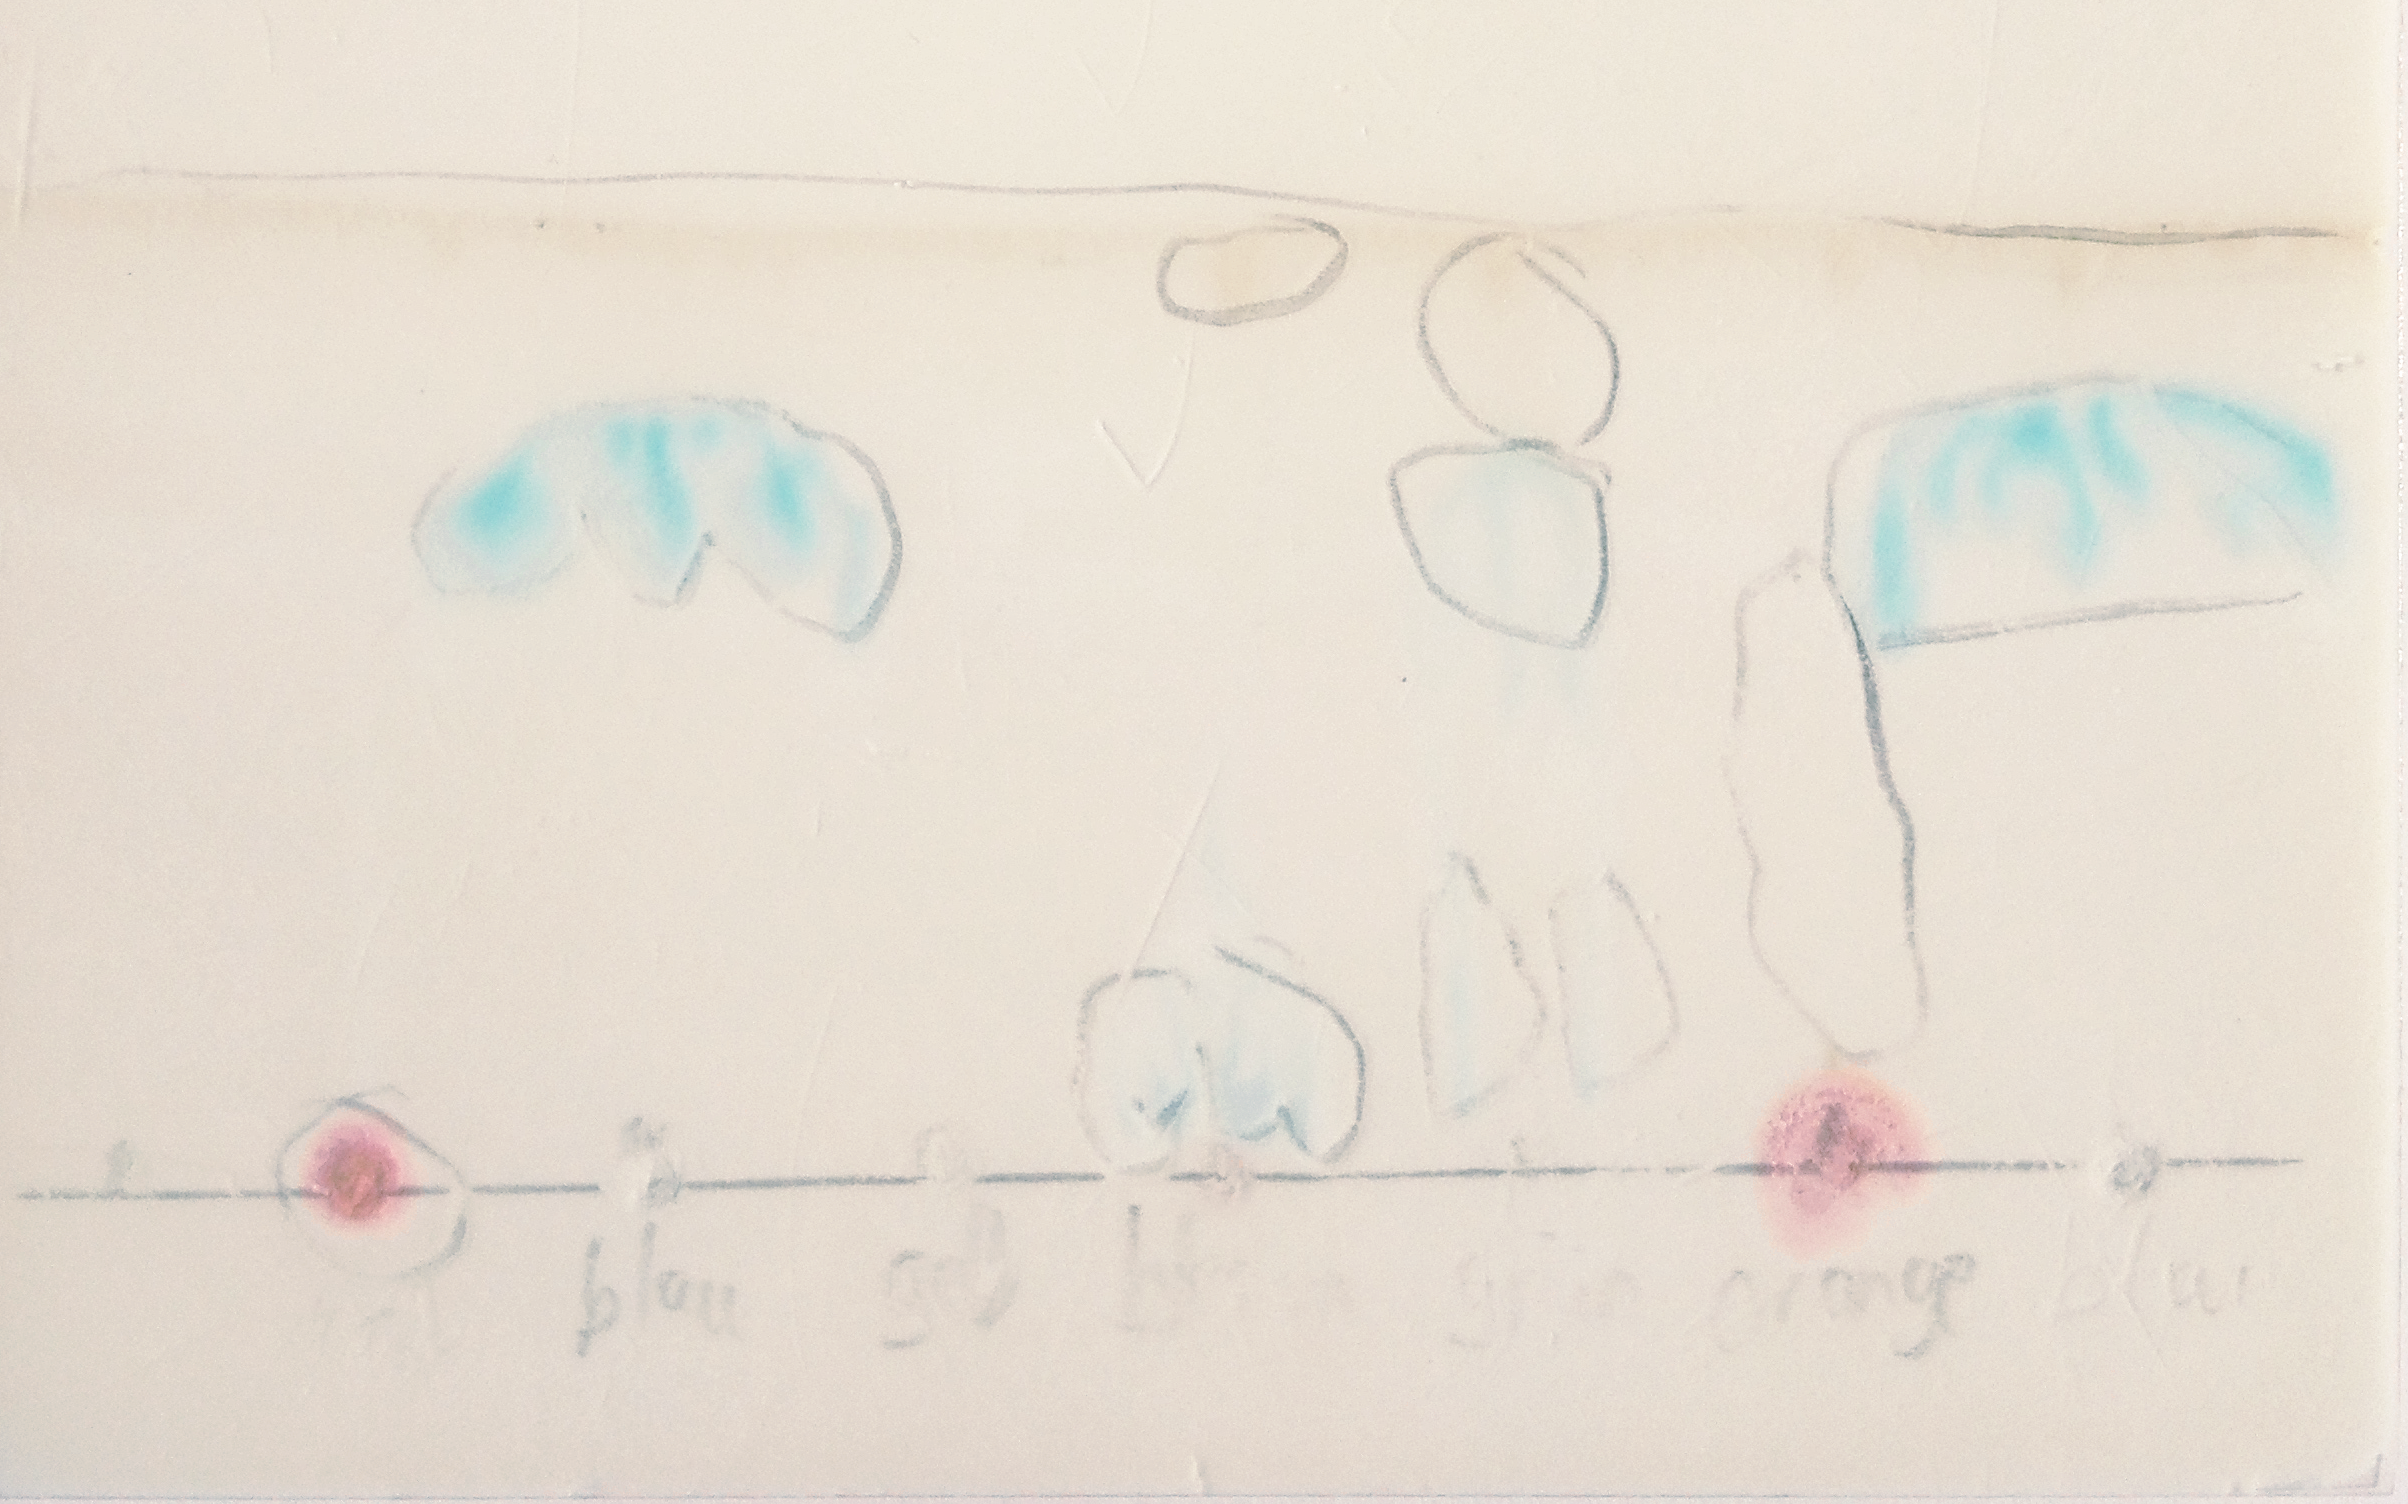
\includegraphics[width=\textwidth]{kieselgel.png}
	\caption{Dünnschichtchromatografie mit Schokolinsen auf einer Kieselgelplatte}
	\label{img: Kieselgel}
\end{figure}

Nach einer Laufzeit von 20 Minuten ist das Laufmittelgemisch, bestehend aus Ethylacetat, Propan-1-ol und Wasser (Verhältniss: 10:60:30) cm an der Kieselgelplatte hochgeflossen.



\begin{figure}[ht!]
\begin{center}
	
	\begin{tikzpicture}
	\begin{axis}[
	draw=none,
	ybar,
	title style={align=center},
	title={Geschmackliche Beurteilung},
	ytick={1, 2.00, 3.00, 4.00, 5.00},
	ylabel=Bewertung,
	xtick=data,
	ymin = 1,
	ymax=5,
axis on top,
height=6cm, width=8cm,
bar width=0.4cm,
ymajorgrids, tick align=inside,
			major grid style={draw=white,line width=1.5pt },
enlarge y limits={value=.1,upper},
enlarge x limits=0.7,
axis x line*=bottom,
axis y line*=left,
y axis line style={opacity=0},
tickwidth=0pt,
legend style={
	at={(0.5,-0.2)},
	anchor=north,
	legend columns=-1,
	/tikz/every even column/.append style={column sep=0.5cm}
},
	symbolic x coords={natürlich,künstlich},
	]
	\addplot[fill=LimeGreen,draw=none] coordinates {(natürlich,3.7) (künstlich, 3.5)};
	\addplot[fill=Goldenrod,draw=none] coordinates {(natürlich,2.9) (künstlich, 3.18)};
	\addplot[fill=BrickRed,draw=none] coordinates {(natürlich,3.7) (künstlich, 3.9)};
	\end{axis}
	\end{tikzpicture}\hfill
	\begin{tikzpicture}
		\begin{axis}[
		draw=none,
		ybar,
		title style={align=center},
		title={Farbigkeit und Aussehen},
		ytick={1, 2.00, 3.00, 4.00, 5.00},
		ylabel=,
		xtick=data,
		ymin = 1,
		ymax=5,
		axis on top,
		height=6cm, width=8cm,
		bar width=0.4cm,
		ymajorgrids, tick align=inside,
			major grid style={draw=white,line width=1.5pt },
		enlarge y limits={value=.1,upper},
		enlarge x limits=0.7,
		axis x line*=bottom,
		axis y line*=left,
		y axis line style={opacity=0},
		tickwidth=0pt,
		legend style={
			at={(0.5,-0.2)},
			anchor=north,
			legend columns=-1,
			/tikz/every even column/.append style={column sep=0.5cm}
		},
		symbolic x coords={natürlich,künstlich},
		]
		\addplot[fill=LimeGreen,draw=none] coordinates {(natürlich,3.63) (künstlich, 3.7)};
		\addplot[fill=Goldenrod,draw=none] coordinates {(natürlich,4.2) (künstlich, 2.9)};
		\addplot[fill=BrickRed,draw=none] coordinates {(natürlich,3.1) (künstlich, 3.7)};
		\end{axis}
		\end{tikzpicture}
		\\[1cm]
		\begin{tikzpicture}
		\pgfplotsset{
			/pgfplots/ybar legend/.style={
				/pgfplots/legend image code/.code={%
					\fill[##1,/tikz/.cd,bar width=3pt,yshift=-0.2em,bar shift=0pt]
					plot coordinates {(0cm,0.8em) (2*\pgfplotbarwidth,0.6em)};},
			}
		}
			\begin{axis}[
			draw=none,
			ybar,
			title style={align=center},
			title={Konsistenz},
			ytick={1, 2.00, 3.00, 4.00, 5.00},
			ylabel=Bewertung,
			xtick=data,
			ymin = 1,
			ymax=5,
			axis on top,
			height=6cm, width=8cm,
			bar width=0.4cm,
			ymajorgrids, tick align=inside,
			major grid style={draw=white,line width=1.5pt },
			enlarge y limits={value=.1,upper},
			enlarge x limits=0.7,
			axis x line*=bottom,
			axis y line*=left,
			y axis line style={opacity=0},
			tickwidth=0pt,
			legend style={
				at={(0.5,-0.2)},
				anchor=north,
				legend columns=-1,
				/tikz/every even column/.append style={column sep=0.5cm}
			},
			symbolic x coords={natürlich,künstlich},
			]
			\addplot[fill=LimeGreen,draw=none] coordinates {(natürlich,3.63) (künstlich, 3.7)};
			\addplot[fill=Goldenrod,draw=none] coordinates {(natürlich,4.2) (künstlich, 2.9)};
			\addplot[fill=BrickRed,draw=none] coordinates {(natürlich,3.1) (künstlich, 3.7)};
			\legend{Grün, Gelb, Rot}
			\end{axis}
			\end{tikzpicture}
\end{center}
\caption[Auswertung der Versuchsreihe mit Lebensmittelfarben]{Auswertung der Versuchsreihe mit gefärbten Muffins. Verwendet wurden sowohl natürliche als auch künstliche Farbstoffe. Die Daten wurden über einen Fragebogen erhoben.}
\label{img:diagram_colors}
\end{figure}


\begin{figure}[htbp]
	\centering
	\includegraphics[width=\textwidth]{Fragebogen.pdf}
	\caption{Fragebogen zur Befragung von Probanden, die mit Lebensmittelfarben behandelte Muffins verkostet hatten.}
	\label{img:questions}
\end{figure}


\printbibliography


\chapter*{Eigenständigkeitserklärung}

Ich habe diese Seminararbeit ohne fremde Hilfe angefertigt und nur die im Literaturverzeichnis angeführten Quellen und Hilfsmittel benutzt.

\vspace{2\baselineskip}
\noindent Neuburg, den \today
\par\noindent\makebox[2.5in]{} \hfill\makebox[2.0in]{\hrulefill}%
\par\noindent\makebox[2.5in][l]{} \hfill\makebox[2.0in][l]{Lukas Braun}

\end{document}